\documentclass[nobib]{tufte-handout}

\title{Föreläsning 7: Dyck-stigar och Catalantal $\cdot$ 1MA020}

\author[Vilhelm Agdur]{Vilhelm Agdur\thanks{\href{mailto:vilhelm.agdur@math.uu.se}{\nolinkurl{vilhelm.agdur@math.uu.se}}}}

%\date{7 februari 2023}


%\geometry{showframe} % display margins for debugging page layout

\usepackage{graphicx} % allow embedded images
  \setkeys{Gin}{width=\linewidth,totalheight=\textheight,keepaspectratio}
  \graphicspath{{graphics/}} % set of paths to search for images
\usepackage{amsmath}  % extended mathematics
\usepackage{booktabs} % book-quality tables
\usepackage{units}    % non-stacked fractions and better unit spacing
\usepackage{multicol} % multiple column layout facilities
\usepackage{lipsum}   % filler text
\usepackage{fancyvrb} % extended verbatim environments
  \fvset{fontsize=\normalsize}% default font size for fancy-verbatim environments

\usepackage{color,soul} % Highlights for text

% Standardize command font styles and environments
\newcommand{\doccmd}[1]{\texttt{\textbackslash#1}}% command name -- adds backslash automatically
\newcommand{\docopt}[1]{\ensuremath{\langle}\textrm{\textit{#1}}\ensuremath{\rangle}}% optional command argument
\newcommand{\docarg}[1]{\textrm{\textit{#1}}}% (required) command argument
\newcommand{\docenv}[1]{\textsf{#1}}% environment name
\newcommand{\docpkg}[1]{\texttt{#1}}% package name
\newcommand{\doccls}[1]{\texttt{#1}}% document class name
\newcommand{\docclsopt}[1]{\texttt{#1}}% document class option name
\newenvironment{docspec}{\begin{quote}\noindent}{\end{quote}}% command specification environment

\include{mathcommands.extratex}

\begin{document}

\definecolor{darkgreen}{rgb}{0.0627, 0.4588, 0.1451}

\maketitle% this prints the handout title, author, and date

\begin{abstract}
\noindent
Vi introducerar Dyck-stigar, och ger två sätt att räkna dem, och ser att bägge ger oss Catalantalen. Sedan ger vi några fler exempel på saker som räknas av Catalantalen.
\end{abstract}

\section{Dyck-stigar}

\begin{definition}
    En \emph{gitterstig} på $\Z^2$ av längd $n$ mellan $a$ och $b$ börjar i punkten $a$ och tar sig sedan till punkten $b$ med $n$ stycken steg, som kan vara upp, ner, höger, eller vänster.\sidenote[][-0.3cm]{Vi kan betrakta en sådan stig som ett ord av längd $n$ ur alfabetet $\{U,N,H,V\}$, tillsammans med en startpunkt.}
    \begin{figure}
        \centering
        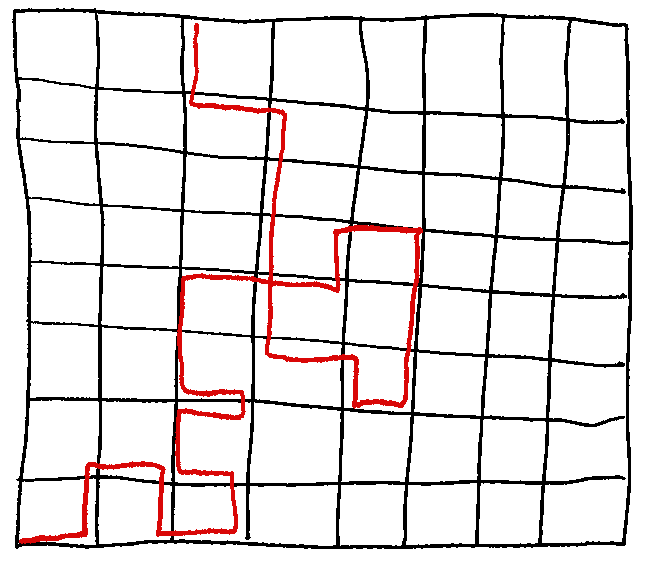
\includegraphics[width=0.5\textwidth]{graphics/general_lattice_path.png}
        \caption{En gitterstig av längd $28$ från $(0,0)$ till $(2,8)$.}
    \end{figure} 
\end{definition}

Det finns uppenbarligen $4^n$ gitterstigar av längd $n$ med en given startpunkt, om vi inte kräver att den skall sluta i någon given punkt.

\begin{definition}
    En \emph{uppåt-höger-stig} på $\Z^2$ från $a$ till $b$ är en gitterstig mellan $a$ och $b$ som enbart tar steg uppåt och åt höger.\sidenote[][]{I tolkningen av stigar som ord är alltså dessa ord ur det mindre alfabetet $\{U,H\}$.}
    \begin{figure}[h]
        \centering
        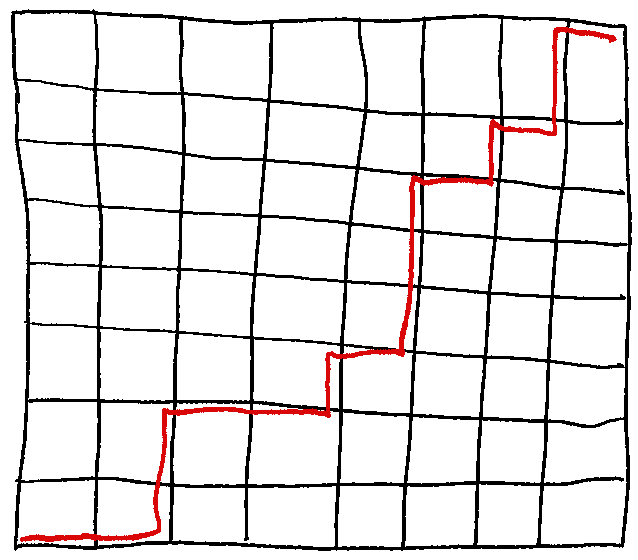
\includegraphics[width=0.5\textwidth]{graphics/right_up_lattice_path.png}
        \caption{En uppåt-höger-stig från $(0,0)$ till $(8,8)$ av längd sexton.}
    \end{figure}
\end{definition}

Notera att till skillnad från allmänna gitterstigar bestäms en uppåt-höger-stigs längd av dess start och slutpunkt, eftersom den inte kan ta några omvägar eller gå baklänges. En stig från $(0,0)$ till $(a,b)$ kommer alltid att ta precis $a$ steg uppåt och $b$ steg till höger, det enda som kan variera är i vilken ording stegen tas.

Alltså ges det totala antalet uppåt-höger-stigar från $(0,0)$ till $(a,b)$ av $\binom{a+b}{a}$, eftersom det är antalet sätt att välja de $a$ ställen vi tar ett steg höger av totalt $a+b$ steg.

\begin{definition}
    En Dyck-stig av längd $2n$ är en uppåt-höger-stig från $(0,0)$ till $(n,n)$ som aldrig går under diagonalen.
    \begin{figure}
        \centering
        \includegraphics*[width=0.5\textwidth]{graphics/Dyck_path.png}
        \caption{En Dyck-stig av längd sexton.}
    \end{figure}
\end{definition}

Notera att en Dyck-stig alltid måste börja med ett steg uppåt och sluta med ett steg åt höger, eftersom den annars ju hade varit under diagonalen.

Hur många Dyck-stigar finns det av varje given längd? Vi kan använda vår observation om att de alltid börjar med ett upp-steg för att ge en rekursion för detta antal:

\begin{lemma}\label{dyck_path_recursion_lemma}
    Låt $d_n$ beteckna antalet Dyck-stigar av längd $2n$. Då gäller det för alla $n \geq 0$ att
    $$d_{n+1} = \sum_{k=0}^{n} d_k d_{n-k}$$
    och $d_0 = 1$.\sidenote[][]{Antalet ord av längd noll anser vi vara ett, eftersom det bara finns ett sätt att välja ett sådant.}

    \begin{proof}
        Överväg en Dyck-stig av längd $2(n+1)$. Vi kan dela upp den i två kortare Dyck-stigar som följer: Den börjar med ett upp-steg, som vi färgar grått. Sedan fortsätter den i ett tag tills den träffar diagonalen för första gången. Vi färgar alla steg innan det steg i vilken den träffar diagonalen röda, och steget i vilken den träffar diagonalen grått. Sedan färgar vi resten av stegen blåa.

        \begin{figure}
            \centering
            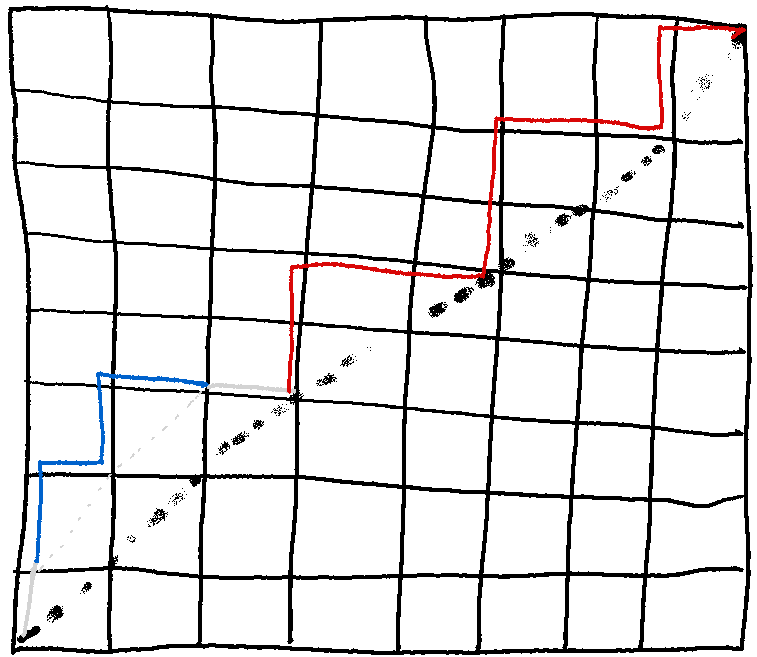
\includegraphics[width = 0.6\textwidth]{graphics/Dyck_path_recursion.png}
            \caption{En illustration av vår uppdelning av en Dyck-stig i gråa, blåa, och röda steg.}
        \end{figure}

        Vi hävdar att de blå stegen utgör en Dyck-stig av längd $2k$ för något $0 \leq k \leq n$, och de röda stegen utgör en Dyck-stig av längd $2(n-k)$, så att vi tillsammans med de två gråa stegen har totalt $2k + 2(n-k) + 2 = 2(n+1)$ steg. Ekvivalent, i tolkningen av stigar som ord, så säger vi att ordet för stigen vi började med kan skrivas som
        $$Uw_1Hw_2$$
        för två kortare\sidenote[][]{Det är tillåtet att de är av längd noll.} Dyck-stigar $w_1$ och $w_2$.

        Vi kan välja $k$ fritt mellan $0$ och $n$, och vi kan sedan välja våra två kortare Dyck-stigar helt fritt så länge de har rätt längd, så multiplikations- och additionsprincipen ger oss att vi kan totalt välja på
        $$\sum_{k=0}^{n} d_k d_{n-k}$$
        sätt, vilket är vad vi ville bevisa.
    \end{proof}
\end{lemma}

Den uppmärksamme bland er kanske redan känt igen att den här rekursionen säger något om en faltning -- specifikt säger den att
$$d_{n+1} = (d * d)_n,$$
vilket ser ut som något vi borde kunna använda för att räkna ut genererande funktionen av den här följden.

\begin{proposition}
    Den genererande funktionen för $\{d_k\}_{k=0}^\infty$, antalet Dyck-stigar, är
    $$F_d(x) = \frac{1 - \sqrt{1 - 4x}}{2x}.$$

    \begin{proof}
        Vi observerar att Lemma \ref{dyck_path_recursion_lemma} ger oss att för alla $n \geq 0$
        $$d_{n+1} = (d*d)_n,$$
        så om vi tar genererande funktioner av bägge sidorna ser vi att vänster led blir
        $$\sum_{n=0}^{\infty}d_{n+1}x^n = \frac{1}{x}\sum_{n=1}^{\infty} d_n x^n = \frac{F_d(x) - 1}{x}$$
        och höger led blir
        $$F_{d * d}(x) = F_d(x)^2$$
        så att vi har att
        $$F_d(x) = x F_d(x)^2 + 1.$$

        Det här är ju bara en vanlig andragradsekvation som vi kan lösa för $F_d$, och få att
        $$F_d(x) = \frac{1 \pm \sqrt{1 - 4x}}{2x}.$$

        Det enda som återstår är att se om den rätta lösningen har ett plus- eller minustecken. Sättet vi ser detta på är att vi vet vad den skall ta för värde i en specifik punkt -- vi kan ju nämligen räkna att
        $$F_d(0) = \sum_{k=0}^{\infty} d_k 0^k = d_0 = 1$$
        så funktionen måste vara ett i noll.

        En snabb räkning ger oss att
        $$\lim_{x \to 0} \frac{1 - \sqrt{1 - 4x}}{2x} = 1$$
        emedan gränsvärdet
        $$\lim_{x \to 0} \frac{1 + \sqrt{1 - 4x}}{2x}$$
        inte existerar. Alltså måste den korrekta lösningen vara med minustecknet, såsom önskat.
    \end{proof}
\end{proposition}

\section{Övningar}

\begin{xca}
    Hur många gitterstigar av längd $n$ från $(0,0)$ till $(a,b)$ finns det?
\end{xca}

%\bibliography{references}
%\bibliographystyle{plainnat}

\end{document}
